% Created by tikzDevice version 0.10.1 on 2016-06-29 14:25:44
% !TEX encoding = UTF-8 Unicode
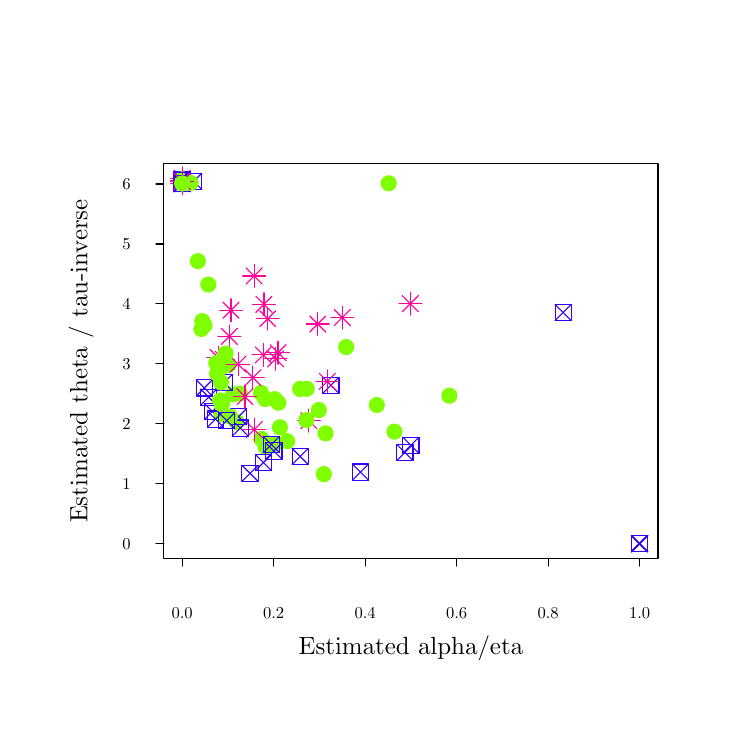
\begin{tikzpicture}[x=1pt,y=1pt]
\definecolor{fillColor}{RGB}{255,255,255}
\path[use as bounding box,fill=fillColor,fill opacity=0.00] (0,0) rectangle (252.94,252.94);
\begin{scope}
\path[clip] ( 49.20, 61.20) rectangle (227.75,203.75);
\definecolor{fillColor}{RGB}{128,255,0}

\path[fill=fillColor] ( 65.27,160.12) circle (  2.92);
\definecolor{drawColor}{RGB}{255,0,153}

\path[draw=drawColor,line width= 0.4pt,line join=round,line cap=round] ( 67.72,130.20) -- ( 73.57,136.05);

\path[draw=drawColor,line width= 0.4pt,line join=round,line cap=round] ( 67.72,136.05) -- ( 73.57,130.20);

\path[draw=drawColor,line width= 0.4pt,line join=round,line cap=round] ( 66.51,133.12) -- ( 74.79,133.12);

\path[draw=drawColor,line width= 0.4pt,line join=round,line cap=round] ( 70.65,128.99) -- ( 70.65,137.26);
\definecolor{drawColor}{RGB}{51,0,255}

\path[draw=drawColor,line width= 0.4pt,line join=round,line cap=round] (218.21, 63.55) rectangle (224.06, 69.40);

\path[draw=drawColor,line width= 0.4pt,line join=round,line cap=round] (218.21, 63.55) -- (224.06, 69.40);

\path[draw=drawColor,line width= 0.4pt,line join=round,line cap=round] (218.21, 69.40) -- (224.06, 63.55);

\path[draw=drawColor,line width= 0.4pt,line join=round,line cap=round] (106.64,120.80) rectangle (112.49,126.65);

\path[draw=drawColor,line width= 0.4pt,line join=round,line cap=round] (106.64,120.80) -- (112.49,126.65);

\path[draw=drawColor,line width= 0.4pt,line join=round,line cap=round] (106.64,126.65) -- (112.49,120.80);

\path[fill=fillColor] ( 84.30,120.99) circle (  2.92);

\path[draw=drawColor,line width= 0.4pt,line join=round,line cap=round] ( 60.90,119.83) rectangle ( 66.75,125.68);

\path[draw=drawColor,line width= 0.4pt,line join=round,line cap=round] ( 60.90,119.83) -- ( 66.75,125.68);

\path[draw=drawColor,line width= 0.4pt,line join=round,line cap=round] ( 60.90,125.68) -- ( 66.75,119.83);

\path[fill=fillColor] ( 89.36,102.57) circle (  2.92);

\path[fill=fillColor] (130.46,196.70) circle (  2.92);

\path[fill=fillColor] ( 90.59,117.40) circle (  2.92);
\definecolor{drawColor}{RGB}{255,0,153}

\path[draw=drawColor,line width= 0.4pt,line join=round,line cap=round] ( 65.90,130.77) -- ( 71.75,136.62);

\path[draw=drawColor,line width= 0.4pt,line join=round,line cap=round] ( 65.90,136.62) -- ( 71.75,130.77);

\path[draw=drawColor,line width= 0.4pt,line join=round,line cap=round] ( 64.69,133.69) -- ( 72.96,133.69);

\path[draw=drawColor,line width= 0.4pt,line join=round,line cap=round] ( 68.83,129.56) -- ( 68.83,137.83);

\path[fill=fillColor] ( 55.81,197.41) circle (  2.92);

\path[fill=fillColor] ( 84.47,104.36) circle (  2.92);

\path[fill=fillColor] ( 56.45,197.12) circle (  2.92);

\path[fill=fillColor] ( 74.23,120.45) circle (  2.92);
\definecolor{drawColor}{RGB}{51,0,255}

\path[draw=drawColor,line width= 0.4pt,line join=round,line cap=round] ( 52.89,194.63) rectangle ( 58.74,200.48);

\path[draw=drawColor,line width= 0.4pt,line join=round,line cap=round] ( 52.89,194.63) -- ( 58.74,200.48);

\path[draw=drawColor,line width= 0.4pt,line join=round,line cap=round] ( 52.89,200.48) -- ( 58.74,194.63);

\path[draw=drawColor,line width= 0.4pt,line join=round,line cap=round] ( 52.89,194.60) rectangle ( 58.74,200.45);

\path[draw=drawColor,line width= 0.4pt,line join=round,line cap=round] ( 52.89,194.60) -- ( 58.74,200.45);

\path[draw=drawColor,line width= 0.4pt,line join=round,line cap=round] ( 52.89,200.45) -- ( 58.74,194.60);
\definecolor{drawColor}{RGB}{255,0,153}

\path[draw=drawColor,line width= 0.4pt,line join=round,line cap=round] (101.89,142.93) -- (107.74,148.78);

\path[draw=drawColor,line width= 0.4pt,line join=round,line cap=round] (101.89,148.78) -- (107.74,142.93);

\path[draw=drawColor,line width= 0.4pt,line join=round,line cap=round] (100.68,145.86) -- (108.95,145.86);

\path[draw=drawColor,line width= 0.4pt,line join=round,line cap=round] (104.82,141.72) -- (104.82,149.99);
\definecolor{drawColor}{RGB}{51,0,255}

\path[draw=drawColor,line width= 0.4pt,line join=round,line cap=round] ( 62.47,116.50) rectangle ( 68.32,122.35);

\path[draw=drawColor,line width= 0.4pt,line join=round,line cap=round] ( 62.47,116.50) -- ( 68.32,122.35);

\path[draw=drawColor,line width= 0.4pt,line join=round,line cap=round] ( 62.47,122.35) -- ( 68.32,116.50);
\definecolor{drawColor}{RGB}{255,0,153}

\path[draw=drawColor,line width= 0.4pt,line join=round,line cap=round] ( 98.67,108.01) -- (104.52,113.86);

\path[draw=drawColor,line width= 0.4pt,line join=round,line cap=round] ( 98.67,113.86) -- (104.52,108.01);

\path[draw=drawColor,line width= 0.4pt,line join=round,line cap=round] ( 97.45,110.93) -- (105.73,110.93);

\path[draw=drawColor,line width= 0.4pt,line join=round,line cap=round] (101.59,106.80) -- (101.59,115.07);
\definecolor{drawColor}{RGB}{51,0,255}

\path[draw=drawColor,line width= 0.4pt,line join=round,line cap=round] ( 52.89,193.75) rectangle ( 58.74,199.60);

\path[draw=drawColor,line width= 0.4pt,line join=round,line cap=round] ( 52.89,193.75) -- ( 58.74,199.60);

\path[draw=drawColor,line width= 0.4pt,line join=round,line cap=round] ( 52.89,199.60) -- ( 58.74,193.75);

\path[draw=drawColor,line width= 0.4pt,line join=round,line cap=round] (218.09, 63.55) rectangle (223.94, 69.40);

\path[draw=drawColor,line width= 0.4pt,line join=round,line cap=round] (218.09, 63.55) -- (223.94, 69.40);

\path[draw=drawColor,line width= 0.4pt,line join=round,line cap=round] (218.09, 69.40) -- (223.94, 63.55);

\path[fill=fillColor] ( 76.68,120.70) circle (  2.92);

\path[fill=fillColor] ( 69.50,129.74) circle (  2.92);
\definecolor{drawColor}{RGB}{255,0,153}

\path[draw=drawColor,line width= 0.4pt,line join=round,line cap=round] ( 52.89,195.54) -- ( 58.74,201.39);

\path[draw=drawColor,line width= 0.4pt,line join=round,line cap=round] ( 52.89,201.39) -- ( 58.74,195.54);

\path[draw=drawColor,line width= 0.4pt,line join=round,line cap=round] ( 51.68,198.47) -- ( 59.95,198.47);

\path[draw=drawColor,line width= 0.4pt,line join=round,line cap=round] ( 55.81,194.33) -- ( 55.81,202.60);
\definecolor{drawColor}{RGB}{51,0,255}

\path[draw=drawColor,line width= 0.4pt,line join=round,line cap=round] ( 63.79,111.31) rectangle ( 69.64,117.16);

\path[draw=drawColor,line width= 0.4pt,line join=round,line cap=round] ( 63.79,111.31) -- ( 69.64,117.16);

\path[draw=drawColor,line width= 0.4pt,line join=round,line cap=round] ( 63.79,117.16) -- ( 69.64,111.31);
\definecolor{drawColor}{RGB}{255,0,153}

\path[draw=drawColor,line width= 0.4pt,line join=round,line cap=round] ( 52.89,194.66) -- ( 58.74,200.51);

\path[draw=drawColor,line width= 0.4pt,line join=round,line cap=round] ( 52.89,200.51) -- ( 58.74,194.66);

\path[draw=drawColor,line width= 0.4pt,line join=round,line cap=round] ( 51.68,197.59) -- ( 59.95,197.59);

\path[draw=drawColor,line width= 0.4pt,line join=round,line cap=round] ( 55.81,193.45) -- ( 55.81,201.73);

\path[fill=fillColor] ( 61.52,168.59) circle (  2.92);
\definecolor{drawColor}{RGB}{51,0,255}

\path[draw=drawColor,line width= 0.4pt,line join=round,line cap=round] (218.21, 63.55) rectangle (224.06, 69.40);

\path[draw=drawColor,line width= 0.4pt,line join=round,line cap=round] (218.21, 63.55) -- (224.06, 69.40);

\path[draw=drawColor,line width= 0.4pt,line join=round,line cap=round] (218.21, 69.40) -- (224.06, 63.55);

\path[fill=fillColor] ( 63.90,145.41) circle (  2.92);

\path[fill=fillColor] ( 89.26,118.70) circle (  2.92);
\definecolor{drawColor}{RGB}{255,0,153}

\path[draw=drawColor,line width= 0.4pt,line join=round,line cap=round] ( 78.46,123.54) -- ( 84.31,129.39);

\path[draw=drawColor,line width= 0.4pt,line join=round,line cap=round] ( 78.46,129.39) -- ( 84.31,123.54);

\path[draw=drawColor,line width= 0.4pt,line join=round,line cap=round] ( 77.24,126.46) -- ( 85.52,126.46);

\path[draw=drawColor,line width= 0.4pt,line join=round,line cap=round] ( 81.38,122.33) -- ( 81.38,130.60);

\path[fill=fillColor] ( 75.51,110.46) circle (  2.92);

\path[fill=fillColor] ( 85.88,101.53) circle (  2.92);

\path[draw=drawColor,line width= 0.4pt,line join=round,line cap=round] ( 69.96,138.46) -- ( 75.81,144.31);

\path[draw=drawColor,line width= 0.4pt,line join=round,line cap=round] ( 69.96,144.31) -- ( 75.81,138.46);

\path[draw=drawColor,line width= 0.4pt,line join=round,line cap=round] ( 68.75,141.38) -- ( 77.03,141.38);

\path[draw=drawColor,line width= 0.4pt,line join=round,line cap=round] ( 72.89,137.24) -- ( 72.89,145.52);

\path[fill=fillColor] (107.02, 91.62) circle (  2.92);
\definecolor{drawColor}{RGB}{51,0,255}

\path[draw=drawColor,line width= 0.4pt,line join=round,line cap=round] (218.21, 63.55) rectangle (224.06, 69.40);

\path[draw=drawColor,line width= 0.4pt,line join=round,line cap=round] (218.21, 63.55) -- (224.06, 69.40);

\path[draw=drawColor,line width= 0.4pt,line join=round,line cap=round] (218.21, 69.40) -- (224.06, 63.55);

\path[fill=fillColor] (105.22,114.77) circle (  2.92);

\path[draw=drawColor,line width= 0.4pt,line join=round,line cap=round] ( 52.89,195.12) rectangle ( 58.74,200.97);

\path[draw=drawColor,line width= 0.4pt,line join=round,line cap=round] ( 52.89,195.12) -- ( 58.74,200.97);

\path[draw=drawColor,line width= 0.4pt,line join=round,line cap=round] ( 52.89,200.97) -- ( 58.74,195.12);

\path[draw=drawColor,line width= 0.4pt,line join=round,line cap=round] (117.35, 89.42) rectangle (123.20, 95.27);

\path[draw=drawColor,line width= 0.4pt,line join=round,line cap=round] (117.35, 89.42) -- (123.20, 95.27);

\path[draw=drawColor,line width= 0.4pt,line join=round,line cap=round] (117.35, 95.27) -- (123.20, 89.42);

\path[draw=drawColor,line width= 0.4pt,line join=round,line cap=round] (133.40, 96.50) rectangle (139.25,102.35);

\path[draw=drawColor,line width= 0.4pt,line join=round,line cap=round] (133.40, 96.50) -- (139.25,102.35);

\path[draw=drawColor,line width= 0.4pt,line join=round,line cap=round] (133.40,102.35) -- (139.25, 96.50);

\path[draw=drawColor,line width= 0.4pt,line join=round,line cap=round] ( 68.06,121.82) rectangle ( 73.91,127.67);

\path[draw=drawColor,line width= 0.4pt,line join=round,line cap=round] ( 68.06,121.82) -- ( 73.91,127.67);

\path[draw=drawColor,line width= 0.4pt,line join=round,line cap=round] ( 68.06,127.67) -- ( 73.91,121.82);

\path[fill=fillColor] ( 72.52,131.03) circle (  2.92);

\path[draw=drawColor,line width= 0.4pt,line join=round,line cap=round] ( 52.89,194.32) rectangle ( 58.74,200.17);

\path[draw=drawColor,line width= 0.4pt,line join=round,line cap=round] ( 52.89,194.32) -- ( 58.74,200.17);

\path[draw=drawColor,line width= 0.4pt,line join=round,line cap=round] ( 52.89,200.17) -- ( 58.74,194.32);

\path[draw=drawColor,line width= 0.4pt,line join=round,line cap=round] ( 52.89,195.15) rectangle ( 58.74,201.00);

\path[draw=drawColor,line width= 0.4pt,line join=round,line cap=round] ( 52.89,195.15) -- ( 58.74,201.00);

\path[draw=drawColor,line width= 0.4pt,line join=round,line cap=round] ( 52.89,201.00) -- ( 58.74,195.15);
\definecolor{drawColor}{RGB}{255,0,153}

\path[draw=drawColor,line width= 0.4pt,line join=round,line cap=round] ( 73.09,128.44) -- ( 78.94,134.29);

\path[draw=drawColor,line width= 0.4pt,line join=round,line cap=round] ( 73.09,134.29) -- ( 78.94,128.44);

\path[draw=drawColor,line width= 0.4pt,line join=round,line cap=round] ( 71.88,131.37) -- ( 80.16,131.37);

\path[draw=drawColor,line width= 0.4pt,line join=round,line cap=round] ( 76.02,127.23) -- ( 76.02,135.50);

\path[fill=fillColor] ( 93.76,103.53) circle (  2.92);

\path[draw=drawColor,line width= 0.4pt,line join=round,line cap=round] ( 86.70,130.32) -- ( 92.55,136.17);

\path[draw=drawColor,line width= 0.4pt,line join=round,line cap=round] ( 86.70,136.17) -- ( 92.55,130.32);

\path[draw=drawColor,line width= 0.4pt,line join=round,line cap=round] ( 85.48,133.25) -- ( 93.76,133.25);

\path[draw=drawColor,line width= 0.4pt,line join=round,line cap=round] ( 89.62,129.11) -- ( 89.62,137.38);

\path[draw=drawColor,line width= 0.4pt,line join=round,line cap=round] (135.34,150.28) -- (141.19,156.13);

\path[draw=drawColor,line width= 0.4pt,line join=round,line cap=round] (135.34,156.13) -- (141.19,150.28);

\path[draw=drawColor,line width= 0.4pt,line join=round,line cap=round] (134.13,153.21) -- (142.41,153.21);

\path[draw=drawColor,line width= 0.4pt,line join=round,line cap=round] (138.27,149.07) -- (138.27,157.34);

\path[fill=fillColor] (126.16,116.59) circle (  2.92);
\definecolor{drawColor}{RGB}{51,0,255}

\path[draw=drawColor,line width= 0.4pt,line join=round,line cap=round] ( 52.89,195.02) rectangle ( 58.74,200.87);

\path[draw=drawColor,line width= 0.4pt,line join=round,line cap=round] ( 52.89,195.02) -- ( 58.74,200.87);

\path[draw=drawColor,line width= 0.4pt,line join=round,line cap=round] ( 52.89,200.87) -- ( 58.74,195.02);
\definecolor{drawColor}{RGB}{255,0,153}

\path[draw=drawColor,line width= 0.4pt,line join=round,line cap=round] ( 78.90,160.29) -- ( 84.75,166.14);

\path[draw=drawColor,line width= 0.4pt,line join=round,line cap=round] ( 78.90,166.14) -- ( 84.75,160.29);

\path[draw=drawColor,line width= 0.4pt,line join=round,line cap=round] ( 77.69,163.22) -- ( 85.96,163.22);

\path[draw=drawColor,line width= 0.4pt,line join=round,line cap=round] ( 81.83,159.08) -- ( 81.83,167.36);

\path[fill=fillColor] ( 70.07,113.18) circle (  2.92);

\path[fill=fillColor] ( 55.81,198.16) circle (  2.92);

\path[draw=drawColor,line width= 0.4pt,line join=round,line cap=round] (105.35,122.20) -- (111.20,128.05);

\path[draw=drawColor,line width= 0.4pt,line join=round,line cap=round] (105.35,128.05) -- (111.20,122.20);

\path[draw=drawColor,line width= 0.4pt,line join=round,line cap=round] (104.14,125.13) -- (112.41,125.13);

\path[draw=drawColor,line width= 0.4pt,line join=round,line cap=round] (108.27,120.99) -- (108.27,129.26);
\definecolor{drawColor}{RGB}{51,0,255}

\path[draw=drawColor,line width= 0.4pt,line join=round,line cap=round] (190.58,147.10) rectangle (196.43,152.95);

\path[draw=drawColor,line width= 0.4pt,line join=round,line cap=round] (190.58,147.10) -- (196.43,152.95);

\path[draw=drawColor,line width= 0.4pt,line join=round,line cap=round] (190.58,152.95) -- (196.43,147.10);

\path[draw=drawColor,line width= 0.4pt,line join=round,line cap=round] ( 52.89,193.58) rectangle ( 58.74,199.43);

\path[draw=drawColor,line width= 0.4pt,line join=round,line cap=round] ( 52.89,193.58) -- ( 58.74,199.43);

\path[draw=drawColor,line width= 0.4pt,line join=round,line cap=round] ( 52.89,199.43) -- ( 58.74,193.58);

\path[draw=drawColor,line width= 0.4pt,line join=round,line cap=round] ( 82.27, 92.88) rectangle ( 88.12, 98.73);

\path[draw=drawColor,line width= 0.4pt,line join=round,line cap=round] ( 82.27, 92.88) -- ( 88.12, 98.73);

\path[draw=drawColor,line width= 0.4pt,line join=round,line cap=round] ( 82.27, 98.73) -- ( 88.12, 92.88);

\path[fill=fillColor] ( 62.77,144.08) circle (  2.92);

\path[draw=drawColor,line width= 0.4pt,line join=round,line cap=round] ( 57.06,194.49) rectangle ( 62.91,200.34);

\path[draw=drawColor,line width= 0.4pt,line join=round,line cap=round] ( 57.06,194.49) -- ( 62.91,200.34);

\path[draw=drawColor,line width= 0.4pt,line join=round,line cap=round] ( 57.06,200.34) -- ( 62.91,194.49);

\path[draw=drawColor,line width= 0.4pt,line join=round,line cap=round] (218.21, 63.55) rectangle (224.06, 69.40);

\path[draw=drawColor,line width= 0.4pt,line join=round,line cap=round] (218.21, 63.55) -- (224.06, 69.40);

\path[draw=drawColor,line width= 0.4pt,line join=round,line cap=round] (218.21, 69.40) -- (224.06, 63.55);
\definecolor{drawColor}{RGB}{255,0,153}

\path[draw=drawColor,line width= 0.4pt,line join=round,line cap=round] ( 87.54,132.55) -- ( 93.39,138.40);

\path[draw=drawColor,line width= 0.4pt,line join=round,line cap=round] ( 87.54,138.40) -- ( 93.39,132.55);

\path[draw=drawColor,line width= 0.4pt,line join=round,line cap=round] ( 86.33,135.47) -- ( 94.60,135.47);

\path[draw=drawColor,line width= 0.4pt,line join=round,line cap=round] ( 90.47,131.34) -- ( 90.47,139.61);
\definecolor{drawColor}{RGB}{51,0,255}

\path[draw=drawColor,line width= 0.4pt,line join=round,line cap=round] ( 86.04, 97.03) rectangle ( 91.89,102.88);

\path[draw=drawColor,line width= 0.4pt,line join=round,line cap=round] ( 86.04, 97.03) -- ( 91.89,102.88);

\path[draw=drawColor,line width= 0.4pt,line join=round,line cap=round] ( 86.04,102.88) -- ( 91.89, 97.03);

\path[draw=drawColor,line width= 0.4pt,line join=round,line cap=round] ( 77.42, 88.99) rectangle ( 83.27, 94.84);

\path[draw=drawColor,line width= 0.4pt,line join=round,line cap=round] ( 77.42, 88.99) -- ( 83.27, 94.84);

\path[draw=drawColor,line width= 0.4pt,line join=round,line cap=round] ( 77.42, 94.84) -- ( 83.27, 88.99);

\path[draw=drawColor,line width= 0.4pt,line join=round,line cap=round] (218.09, 63.55) rectangle (223.94, 69.40);

\path[draw=drawColor,line width= 0.4pt,line join=round,line cap=round] (218.09, 63.55) -- (223.94, 69.40);

\path[draw=drawColor,line width= 0.4pt,line join=round,line cap=round] (218.09, 69.40) -- (223.94, 63.55);

\path[draw=drawColor,line width= 0.4pt,line join=round,line cap=round] ( 73.26,109.43) rectangle ( 79.11,115.28);

\path[draw=drawColor,line width= 0.4pt,line join=round,line cap=round] ( 73.26,109.43) -- ( 79.11,115.28);

\path[draw=drawColor,line width= 0.4pt,line join=round,line cap=round] ( 73.26,115.28) -- ( 79.11,109.43);

\path[fill=fillColor] ( 91.14,108.55) circle (  2.92);

\path[fill=fillColor] ( 85.77,118.76) circle (  2.92);
\definecolor{drawColor}{RGB}{255,0,153}

\path[draw=drawColor,line width= 0.4pt,line join=round,line cap=round] ( 52.89,193.74) -- ( 58.74,199.59);

\path[draw=drawColor,line width= 0.4pt,line join=round,line cap=round] ( 52.89,199.59) -- ( 58.74,193.74);

\path[draw=drawColor,line width= 0.4pt,line join=round,line cap=round] ( 51.68,196.67) -- ( 59.95,196.67);

\path[draw=drawColor,line width= 0.4pt,line join=round,line cap=round] ( 55.81,192.53) -- ( 55.81,200.80);

\path[fill=fillColor] (100.83,122.44) circle (  2.92);

\path[draw=drawColor,line width= 0.4pt,line join=round,line cap=round] ( 78.97,104.76) -- ( 84.82,110.61);

\path[draw=drawColor,line width= 0.4pt,line join=round,line cap=round] ( 78.97,110.61) -- ( 84.82,104.76);

\path[draw=drawColor,line width= 0.4pt,line join=round,line cap=round] ( 77.75,107.68) -- ( 86.03,107.68);

\path[draw=drawColor,line width= 0.4pt,line join=round,line cap=round] ( 81.89,103.55) -- ( 81.89,111.82);
\definecolor{drawColor}{RGB}{51,0,255}

\path[draw=drawColor,line width= 0.4pt,line join=round,line cap=round] ( 73.91,105.31) rectangle ( 79.76,111.16);

\path[draw=drawColor,line width= 0.4pt,line join=round,line cap=round] ( 73.91,105.31) -- ( 79.76,111.16);

\path[draw=drawColor,line width= 0.4pt,line join=round,line cap=round] ( 73.91,111.16) -- ( 79.76,105.31);
\definecolor{drawColor}{RGB}{255,0,153}

\path[draw=drawColor,line width= 0.4pt,line join=round,line cap=round] ( 83.83,144.83) -- ( 89.68,150.68);

\path[draw=drawColor,line width= 0.4pt,line join=round,line cap=round] ( 83.83,150.68) -- ( 89.68,144.83);

\path[draw=drawColor,line width= 0.4pt,line join=round,line cap=round] ( 82.62,147.75) -- ( 90.89,147.75);

\path[draw=drawColor,line width= 0.4pt,line join=round,line cap=round] ( 86.75,143.62) -- ( 86.75,151.89);

\path[fill=fillColor] ( 98.44,122.39) circle (  2.92);

\path[draw=drawColor,line width= 0.4pt,line join=round,line cap=round] ( 75.60,116.66) -- ( 81.45,122.51);

\path[draw=drawColor,line width= 0.4pt,line join=round,line cap=round] ( 75.60,122.51) -- ( 81.45,116.66);

\path[draw=drawColor,line width= 0.4pt,line join=round,line cap=round] ( 74.39,119.58) -- ( 82.66,119.58);

\path[draw=drawColor,line width= 0.4pt,line join=round,line cap=round] ( 78.53,115.45) -- ( 78.53,123.72);

\path[fill=fillColor] (115.09,137.54) circle (  2.92);
\definecolor{drawColor}{RGB}{51,0,255}

\path[draw=drawColor,line width= 0.4pt,line join=round,line cap=round] ( 52.89,193.82) rectangle ( 58.74,199.67);

\path[draw=drawColor,line width= 0.4pt,line join=round,line cap=round] ( 52.89,193.82) -- ( 58.74,199.67);

\path[draw=drawColor,line width= 0.4pt,line join=round,line cap=round] ( 52.89,199.67) -- ( 58.74,193.82);

\path[draw=drawColor,line width= 0.4pt,line join=round,line cap=round] (135.56, 99.11) rectangle (141.41,104.96);

\path[draw=drawColor,line width= 0.4pt,line join=round,line cap=round] (135.56, 99.11) -- (141.41,104.96);

\path[draw=drawColor,line width= 0.4pt,line join=round,line cap=round] (135.56,104.96) -- (141.41, 99.11);

\path[draw=drawColor,line width= 0.4pt,line join=round,line cap=round] ( 64.94,108.57) rectangle ( 70.79,114.42);

\path[draw=drawColor,line width= 0.4pt,line join=round,line cap=round] ( 64.94,108.57) -- ( 70.79,114.42);

\path[draw=drawColor,line width= 0.4pt,line join=round,line cap=round] ( 64.94,114.42) -- ( 70.79,108.57);
\definecolor{drawColor}{RGB}{255,0,153}

\path[draw=drawColor,line width= 0.4pt,line join=round,line cap=round] ( 70.55,147.91) -- ( 76.40,153.76);

\path[draw=drawColor,line width= 0.4pt,line join=round,line cap=round] ( 70.55,153.76) -- ( 76.40,147.91);

\path[draw=drawColor,line width= 0.4pt,line join=round,line cap=round] ( 69.34,150.84) -- ( 77.61,150.84);

\path[draw=drawColor,line width= 0.4pt,line join=round,line cap=round] ( 73.48,146.70) -- ( 73.48,154.97);
\definecolor{drawColor}{RGB}{51,0,255}

\path[draw=drawColor,line width= 0.4pt,line join=round,line cap=round] ( 52.89,194.62) rectangle ( 58.74,200.47);

\path[draw=drawColor,line width= 0.4pt,line join=round,line cap=round] ( 52.89,194.62) -- ( 58.74,200.47);

\path[draw=drawColor,line width= 0.4pt,line join=round,line cap=round] ( 52.89,200.47) -- ( 58.74,194.62);

\path[fill=fillColor] ( 73.17,112.39) circle (  2.92);

\path[fill=fillColor] ( 68.14,131.73) circle (  2.92);
\definecolor{drawColor}{RGB}{255,0,153}

\path[draw=drawColor,line width= 0.4pt,line join=round,line cap=round] ( 82.22,131.78) -- ( 88.07,137.63);

\path[draw=drawColor,line width= 0.4pt,line join=round,line cap=round] ( 82.22,137.63) -- ( 88.07,131.78);

\path[draw=drawColor,line width= 0.4pt,line join=round,line cap=round] ( 81.01,134.71) -- ( 89.29,134.71);

\path[draw=drawColor,line width= 0.4pt,line join=round,line cap=round] ( 85.15,130.57) -- ( 85.15,138.84);

\path[fill=fillColor] ( 58.88,196.84) circle (  2.92);

\path[draw=drawColor,line width= 0.4pt,line join=round,line cap=round] ( 52.89,194.48) -- ( 58.74,200.33);

\path[draw=drawColor,line width= 0.4pt,line join=round,line cap=round] ( 52.89,200.33) -- ( 58.74,194.48);

\path[draw=drawColor,line width= 0.4pt,line join=round,line cap=round] ( 51.68,197.41) -- ( 59.95,197.41);

\path[draw=drawColor,line width= 0.4pt,line join=round,line cap=round] ( 55.81,193.27) -- ( 55.81,201.54);

\path[fill=fillColor] ( 55.81,196.63) circle (  2.92);

\path[fill=fillColor] ( 70.18,116.89) circle (  2.92);
\definecolor{drawColor}{RGB}{51,0,255}

\path[draw=drawColor,line width= 0.4pt,line join=round,line cap=round] ( 85.13, 99.39) rectangle ( 90.98,105.24);

\path[draw=drawColor,line width= 0.4pt,line join=round,line cap=round] ( 85.13, 99.39) -- ( 90.98,105.24);

\path[draw=drawColor,line width= 0.4pt,line join=round,line cap=round] ( 85.13,105.24) -- ( 90.98, 99.39);

\path[fill=fillColor] (132.53,106.98) circle (  2.92);

\path[fill=fillColor] (107.64,106.34) circle (  2.92);

\path[fill=fillColor] ( 71.51,135.19) circle (  2.92);
\definecolor{drawColor}{RGB}{255,0,153}

\path[draw=drawColor,line width= 0.4pt,line join=round,line cap=round] ( 82.46,150.05) -- ( 88.31,155.90);

\path[draw=drawColor,line width= 0.4pt,line join=round,line cap=round] ( 82.46,155.90) -- ( 88.31,150.05);

\path[draw=drawColor,line width= 0.4pt,line join=round,line cap=round] ( 81.25,152.98) -- ( 89.52,152.98);

\path[draw=drawColor,line width= 0.4pt,line join=round,line cap=round] ( 85.38,148.84) -- ( 85.38,157.12);
\definecolor{drawColor}{RGB}{51,0,255}

\path[draw=drawColor,line width= 0.4pt,line join=round,line cap=round] ( 69.01,108.04) rectangle ( 74.86,113.89);

\path[draw=drawColor,line width= 0.4pt,line join=round,line cap=round] ( 69.01,108.04) -- ( 74.86,113.89);

\path[draw=drawColor,line width= 0.4pt,line join=round,line cap=round] ( 69.01,113.89) -- ( 74.86,108.04);
\definecolor{drawColor}{RGB}{255,0,153}

\path[draw=drawColor,line width= 0.4pt,line join=round,line cap=round] (110.76,145.26) -- (116.61,151.11);

\path[draw=drawColor,line width= 0.4pt,line join=round,line cap=round] (110.76,151.11) -- (116.61,145.26);

\path[draw=drawColor,line width= 0.4pt,line join=round,line cap=round] (109.55,148.19) -- (117.82,148.19);

\path[draw=drawColor,line width= 0.4pt,line join=round,line cap=round] (113.68,144.05) -- (113.68,152.33);

\path[fill=fillColor] ( 63.09,146.93) circle (  2.92);

\path[fill=fillColor] ( 69.53,118.25) circle (  2.92);
\definecolor{drawColor}{RGB}{51,0,255}

\path[draw=drawColor,line width= 0.4pt,line join=round,line cap=round] ( 95.54, 95.09) rectangle (101.39,100.94);

\path[draw=drawColor,line width= 0.4pt,line join=round,line cap=round] ( 95.54, 95.09) -- (101.39,100.94);

\path[draw=drawColor,line width= 0.4pt,line join=round,line cap=round] ( 95.54,100.94) -- (101.39, 95.09);

\path[fill=fillColor] (100.71,111.17) circle (  2.92);

\path[fill=fillColor] (152.38,119.95) circle (  2.92);

\path[fill=fillColor] ( 68.44,127.90) circle (  2.92);

\path[fill=fillColor] ( 69.83,124.75) circle (  2.92);
\end{scope}
\begin{scope}
\path[clip] (  0.00,  0.00) rectangle (252.94,252.94);
\definecolor{drawColor}{RGB}{0,0,0}

\path[draw=drawColor,line width= 0.4pt,line join=round,line cap=round] ( 55.81, 61.20) -- (221.13, 61.20);

\path[draw=drawColor,line width= 0.4pt,line join=round,line cap=round] ( 55.81, 61.20) -- ( 55.81, 58.35);

\path[draw=drawColor,line width= 0.4pt,line join=round,line cap=round] ( 88.88, 61.20) -- ( 88.88, 58.35);

\path[draw=drawColor,line width= 0.4pt,line join=round,line cap=round] (121.94, 61.20) -- (121.94, 58.35);

\path[draw=drawColor,line width= 0.4pt,line join=round,line cap=round] (155.00, 61.20) -- (155.00, 58.35);

\path[draw=drawColor,line width= 0.4pt,line join=round,line cap=round] (188.07, 61.20) -- (188.07, 58.35);

\path[draw=drawColor,line width= 0.4pt,line join=round,line cap=round] (221.13, 61.20) -- (221.13, 58.35);

\node[text=drawColor,anchor=base,inner sep=0pt, outer sep=0pt, scale=  0.60] at ( 55.81, 39.60) {0.0};

\node[text=drawColor,anchor=base,inner sep=0pt, outer sep=0pt, scale=  0.60] at ( 88.88, 39.60) {0.2};

\node[text=drawColor,anchor=base,inner sep=0pt, outer sep=0pt, scale=  0.60] at (121.94, 39.60) {0.4};

\node[text=drawColor,anchor=base,inner sep=0pt, outer sep=0pt, scale=  0.60] at (155.00, 39.60) {0.6};

\node[text=drawColor,anchor=base,inner sep=0pt, outer sep=0pt, scale=  0.60] at (188.07, 39.60) {0.8};

\node[text=drawColor,anchor=base,inner sep=0pt, outer sep=0pt, scale=  0.60] at (221.13, 39.60) {1.0};

\path[draw=drawColor,line width= 0.4pt,line join=round,line cap=round] ( 49.20, 66.48) -- ( 49.20,196.44);

\path[draw=drawColor,line width= 0.4pt,line join=round,line cap=round] ( 49.20, 66.48) -- ( 46.35, 66.48);

\path[draw=drawColor,line width= 0.4pt,line join=round,line cap=round] ( 49.20, 88.14) -- ( 46.35, 88.14);

\path[draw=drawColor,line width= 0.4pt,line join=round,line cap=round] ( 49.20,109.80) -- ( 46.35,109.80);

\path[draw=drawColor,line width= 0.4pt,line join=round,line cap=round] ( 49.20,131.46) -- ( 46.35,131.46);

\path[draw=drawColor,line width= 0.4pt,line join=round,line cap=round] ( 49.20,153.12) -- ( 46.35,153.12);

\path[draw=drawColor,line width= 0.4pt,line join=round,line cap=round] ( 49.20,174.78) -- ( 46.35,174.78);

\path[draw=drawColor,line width= 0.4pt,line join=round,line cap=round] ( 49.20,196.44) -- ( 46.35,196.44);

\node[text=drawColor,anchor=base east,inner sep=0pt, outer sep=0pt, scale=  0.60] at ( 37.20, 64.41) {0};

\node[text=drawColor,anchor=base east,inner sep=0pt, outer sep=0pt, scale=  0.60] at ( 37.20, 86.07) {1};

\node[text=drawColor,anchor=base east,inner sep=0pt, outer sep=0pt, scale=  0.60] at ( 37.20,107.73) {2};

\node[text=drawColor,anchor=base east,inner sep=0pt, outer sep=0pt, scale=  0.60] at ( 37.20,129.40) {3};

\node[text=drawColor,anchor=base east,inner sep=0pt, outer sep=0pt, scale=  0.60] at ( 37.20,151.06) {4};

\node[text=drawColor,anchor=base east,inner sep=0pt, outer sep=0pt, scale=  0.60] at ( 37.20,172.72) {5};

\node[text=drawColor,anchor=base east,inner sep=0pt, outer sep=0pt, scale=  0.60] at ( 37.20,194.38) {6};

\path[draw=drawColor,line width= 0.4pt,line join=round,line cap=round] ( 49.20, 61.20) --
	(227.75, 61.20) --
	(227.75,203.75) --
	( 49.20,203.75) --
	( 49.20, 61.20);
\end{scope}
\begin{scope}
\path[clip] (  0.00,  0.00) rectangle (252.94,252.94);
\definecolor{drawColor}{RGB}{0,0,0}

\node[text=drawColor,anchor=base,inner sep=0pt, outer sep=0pt, scale=  0.90] at (138.47, 26.40) {Estimated alpha/eta};

\node[text=drawColor,rotate= 90.00,anchor=base,inner sep=0pt, outer sep=0pt, scale=  0.90] at ( 21.60,132.47) {Estimated theta / tau-inverse};
\end{scope}
\end{tikzpicture}
